\documentclass{standalone}
\usepackage{tikz}
\usetikzlibrary{intersections}
\begin{document}
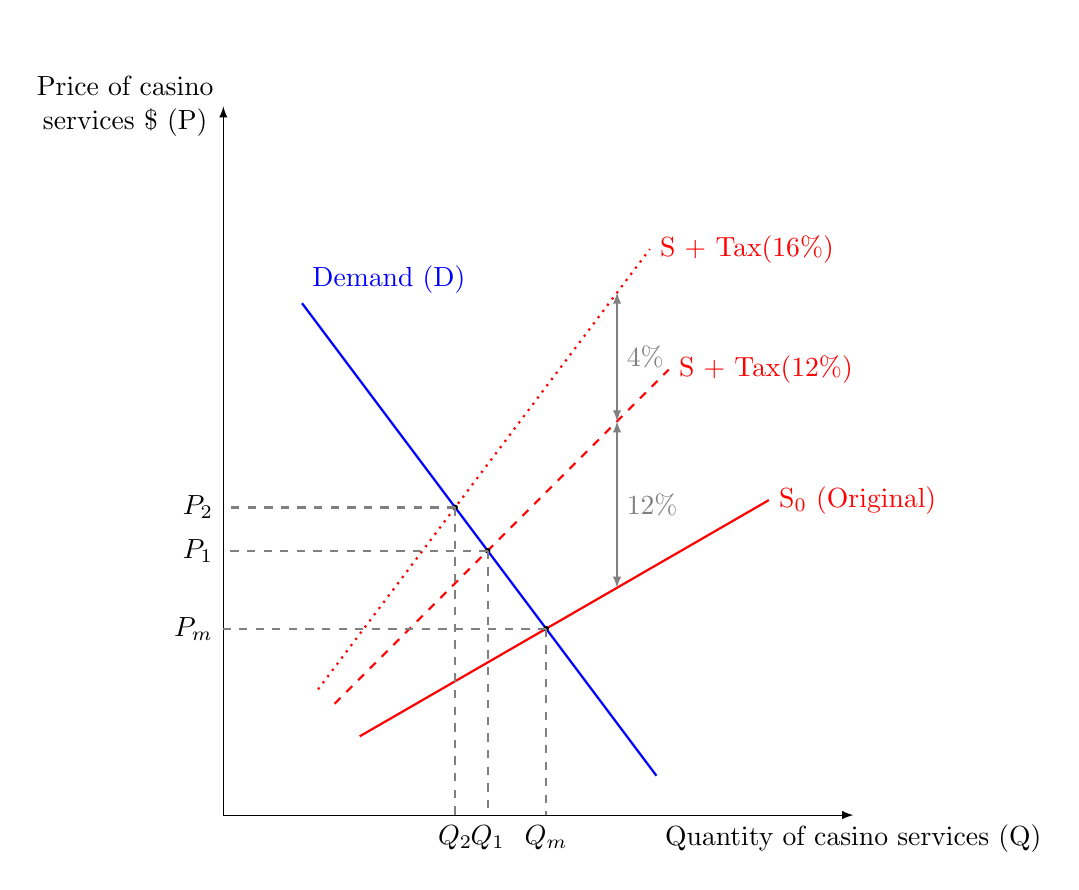
\begin{tikzpicture}[scale=1, >=latex]
    % Axes with padding
    \draw[->] (0,0) -- (8,0) node[below] {Quantity of casino services (Q)};
    \draw[->] (0,0) -- (0,9) node[left, align = center] {Price of casino\\ services $\mathdollar$ (P)};

    % Original supply point (hidden anchor)
    \coordinate (origin) at (0, 0);

    % Supply curves with different slopes through (0.5,2.5)
    \draw[red, thick, name path=s0] (30:2) -- (30:8) node[right] {S\textsubscript{0} (Original)};
    \draw[red, thick, dashed, name path=s1] (45:2) -- (45:8) node[right] {S + Tax(12\%)};
    \draw[red, thick, dotted, name path=s2] (53:2) -- (53:9) node[right] {S + Tax(16\%)};

    % Demand curve
    \draw[blue, thick, name path=de] (5.5,0.5) -- (1, 6.5) node[above, above right] {Demand (D)};

    
    \fill[black, name intersections={of=de and s0, by={des0}}]
        (intersection-1) circle (1pt);
    \draw[gray, thick, dashed] (des0) -- (des0 -| 0,0)
        node[black, left] {$P_m$};
    \draw[gray, thick, dashed] (des0) -- (des0 |- 0,0)
        node[black, below] {$Q_m$};
        

    \fill[black, name intersections={of=de and s1, by={des1}}]
        (intersection-1) circle (1pt);
    \draw[gray, thick, dashed] (des1) -- (des1 -| 0,0)
        node[black, left] {$P_1$};
    \draw[gray, thick, dashed] (des1) -- (des1 |- 0,0)
        node[black, below] {$Q_1$};

    \fill[black, name intersections={of=de and s2, by={des2}}]
        (intersection-1) circle (1pt);
    \draw[gray, thick, dashed] (des2) -- (des2 -| 0,0)
        node[black, left] {$P_2$};
    \draw[gray, thick, dashed] (des2) -- (des2 |- 0,0)
        node[black, below] {$Q_2$};
    
    %\draw[gray] (0,10) -- (10,0);
    \path[name path=arr] (5,10) -- (5,0);
    \path[name intersections={of=arr and s0, by={a0}}];
    \path[name intersections={of=arr and s1, by={a1}}];
    \path[name intersections={of=arr and s2, by={a2}}];

    % Tax arrows at Q=4
    \draw[<->, gray] (a0) -- (a1) 
        node[midway, right] {12\%};
    \draw[<->, gray] (a1) -- (a2)
        node[midway, right] {4\%};

\end{tikzpicture}
\end{document}